\documentclass[12pt]{article}

%%%%%%%%%%%%%%%%%%%%%%% Don't change anything in here. This space is called the preamble, it is where you tell the computer to load the proper LaTeX packages to perform the math and formatting desired. 
\usepackage{caption}
\usepackage{physics} 
\usepackage{siunitx} 
\usepackage{enumerate} 
\usepackage{pgfplots}
\usepackage{pgfplotstable}
\usepackage{tikz,pgfplots}
\usepackage{amsmath}  %I added this so that you can use the align tool for equations!
\usepackage{wasysym} %This package allows you to put emojis in your paper!!!!
	%wasysym: \smiley{} \frownie{} see http://milde.users.sourceforge.net/LUCR/Math/mathpackages/wasysym-symbols.pdf for list of most symbols available in this package
\usepackage{float}
\usepackage{geometry}
 \geometry{
 a4paper,
 total={170mm,257mm},
 left=20mm,
 top=20mm,
 }

\pgfplotsset{compat=1.14}
%%%%%%%%%%%%%%%%%%%%%%%%% Again, Don't change anything Above %%%%%%%%%%%%%%%%%%%%

\begin{document}

\title{The grating monochromator} %Title should be concise and to the point  
\author{JINTIAN WANG, Exeter College, Oxford} %Your name first


\date{\today}  % This will automatically put today's date in the report

\maketitle  %this command makes the title

%%%% to use this template, please copy-paste the entire thing into a new document and save it so you have it!

%%%%% If you want to omit something in this lab, place a % sign to the left of it and it won't show up on the lab, like this line!

\begin{abstract} 
1
\end{abstract}

\section{Introduction}

As quantum theory developed, energy levels of atoms were found to be quantized, and the emission spectra of atoms were found to consist of discrete lines. By measuring the wavelengths of these lines, the energy levels of atoms could be determined, and we can verify the predictions of quantum theory. In this experiment, we will use a Czerny-Turner monochromator to measure the emission spectrum of a mercury lamp, and determine the energy levels of mercury atoms. Then we will use the same monochromator to measure the emission spectrum of a hydrogen lamp, and determine the wavelengths each emission line corresponds to.

\section{Theory}

In the Czerny-Turner monochromator, concave mirrors are used to collimate the beam of light falling on the grating and to focus those beams diffracted from the grating, as shown in figure \ref{fig1}.


\begin{figure}[htbp]
\centering

\begin{minipage}{0.48\textwidth}
    \centering
    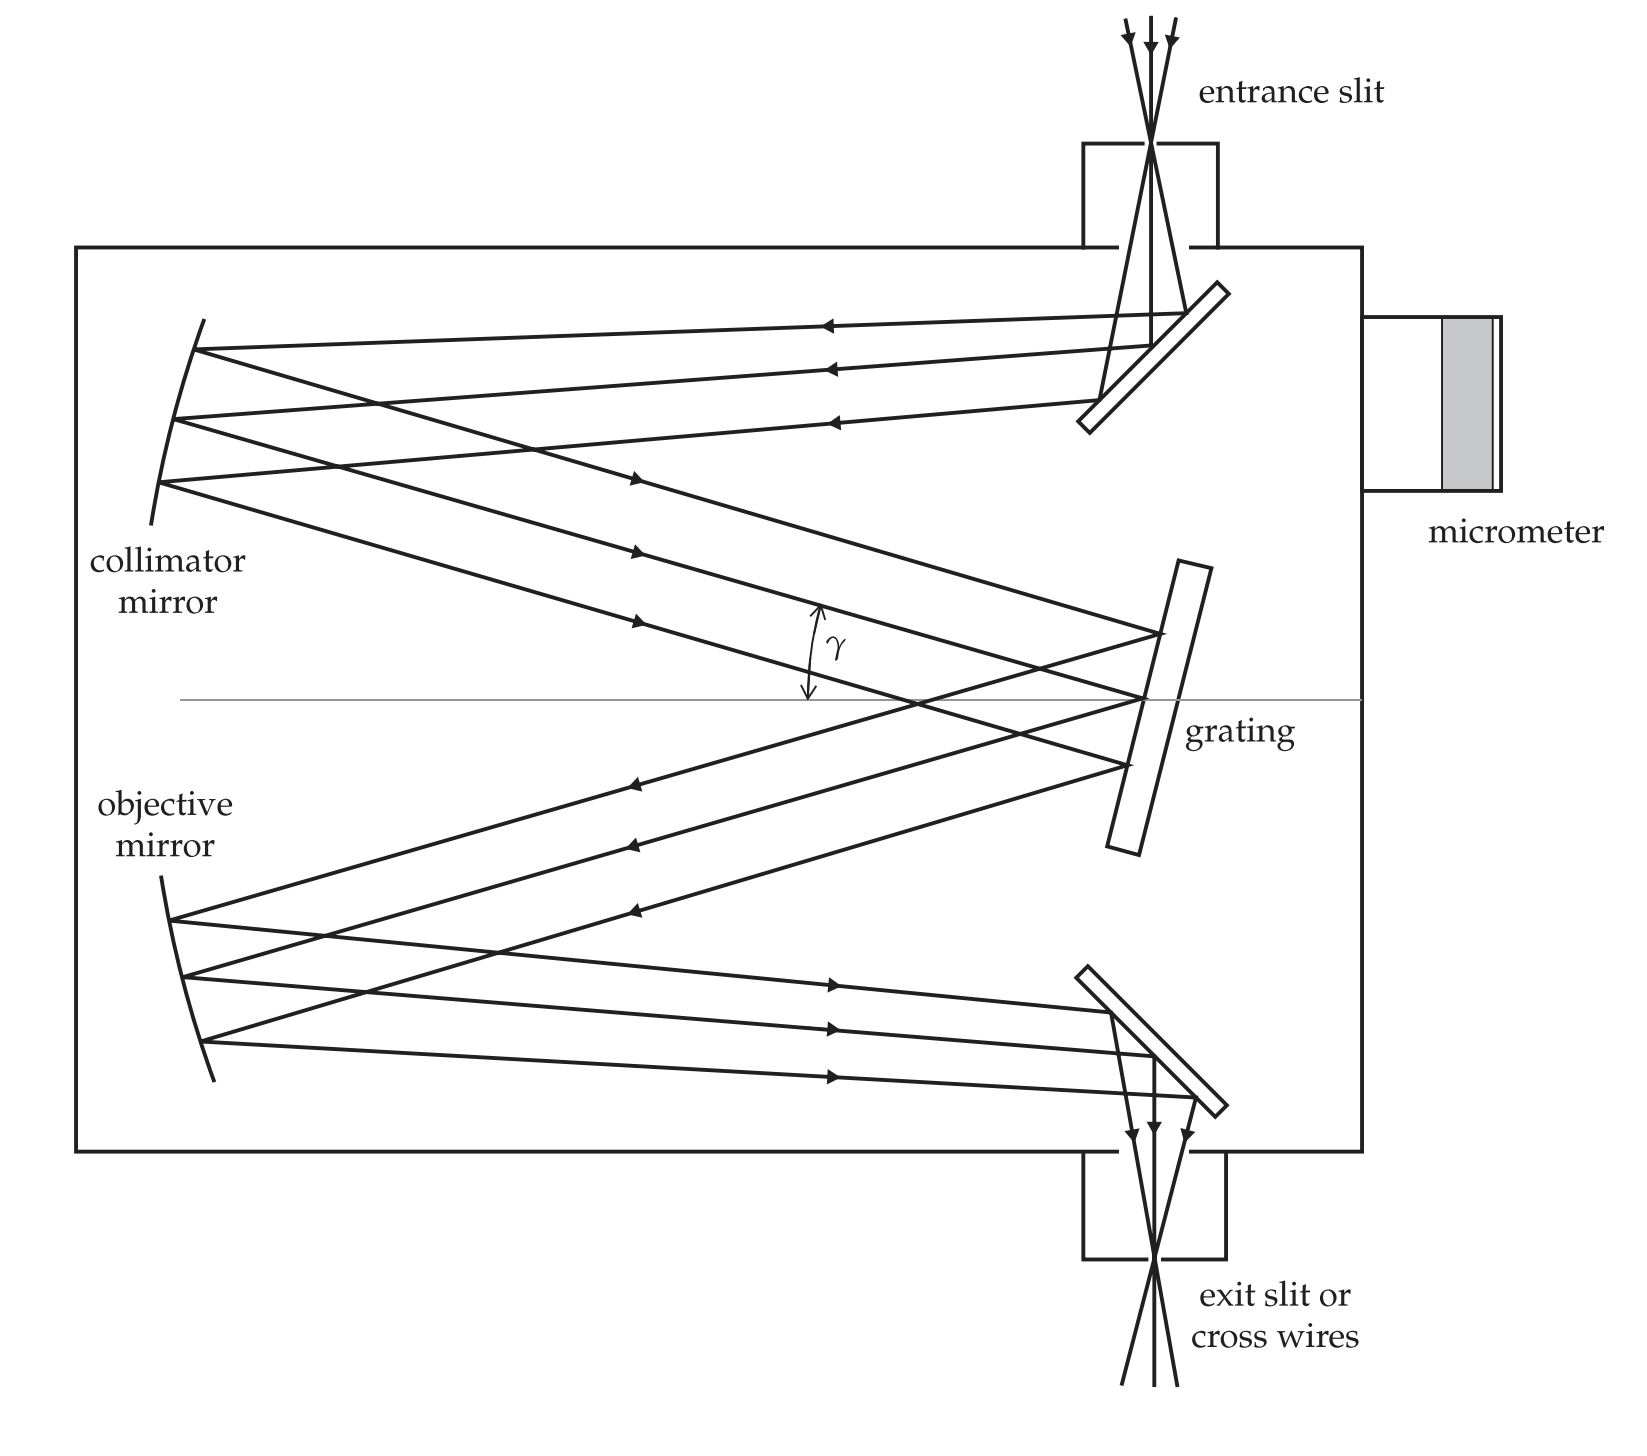
\includegraphics[width=0.9\textwidth]{monochromator.png}
    \captionof{figure}{Czerny--Turner monochromator.}
    \label{fig1}
\end{minipage}
\hfill
\begin{minipage}{0.48\textwidth}
    \centering
    \begin{tabular}{|l|r|}
    \hline
    Grating size & 48\,mm $\times$ 48\,mm \\ \hline
    Ruling frequency $(1/d)$ & 1200\,lines/mm \\ \hline
    Mirror diameter & 63.5\,mm \\ \hline
    Mirror radius of curvature & 439\,mm \\ \hline
    Czerny--Turner angle, $\gamma$ & $25^\circ 28'$ \\ \hline
    Length of sine-bar, $l$ & 75.24\,mm \\ \hline
    \end{tabular}
    \captionof{table}{Design parameters of the Czerny-Turner monochromator.}
    \label{tb1}
\end{minipage}

\end{figure}


According to \cite{op13}, the wavelength $\lambda$ of the light diffracted by the grating is given by
\begin{equation}
\lambda = z\left( \frac{2d\cos\gamma}{pl} \right),
\end{equation}
where $z$ is the reading on the sine-bar, $d$ is the grating spacing, $\gamma$ is the Czerny--Turner angle, $p$ is the ruling frequency of the grating, and $l$ is the length of the sine-bar. Take the data in table \ref{tb1}, we can calculate coefficient $2d\cos\gamma/pl=2.000 \times 10^{-5}$.


\section{Experimental Setup}

\subsection{Calibration}

The monochromator was calibrated using the known vacuum wavelengths of the mercury emission spectrum. 
Although the sine-bar mechanism provides an approximately linear relation between micrometer reading $z$ and wavelength $\lambda$, mechanical imperfections and backlash in the drive mean that an empirical calibration is required.

With the mercury lamp aligned as described in figure \ref{spectra}, each visible spectral line was brought into coincidence with the cross-hair in the exit aperture. For each line, the micrometer was always approached from the same direction to eliminate backlash errors in the sine-bar mechanism.

\begin{figure}[htbp]
\centering

\includegraphics[width=0.9\textwidth]{output.png}
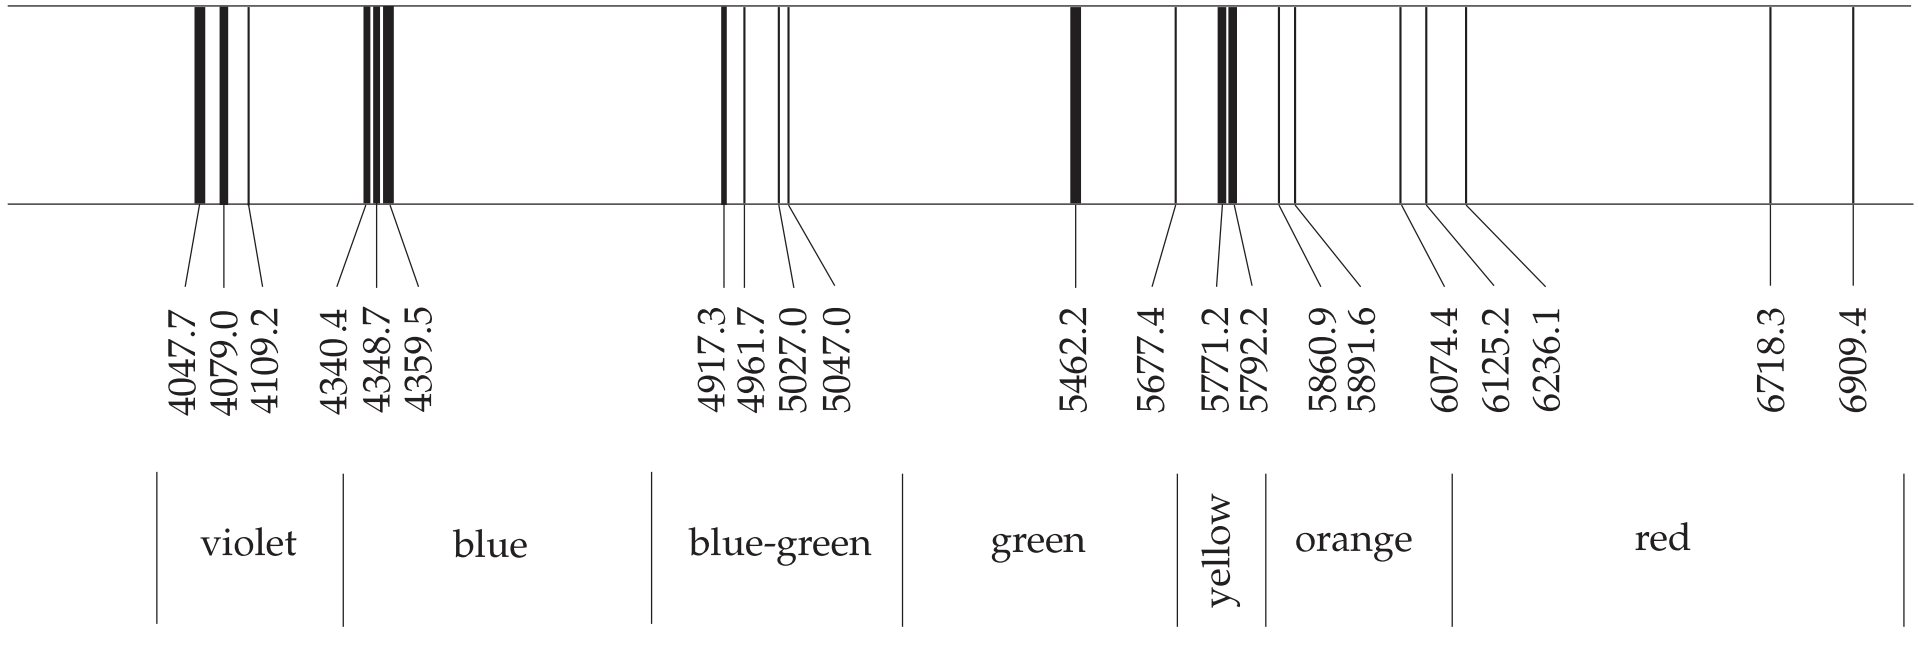
\includegraphics[width=0.9\textwidth]{mer.png}
\caption{Corresponding mercury spectrum \cite{op13}}
\label{spectra}
\end{figure}


Three readings were taken for each spectral line and averaged. The data were recorded in table \ref{calibration}. The slit width was kept fixed throughout the calibration procedure and was not altered subsequently, in order to avoid systematic shifts in the apparent line centre.

The averaged micrometer readings were then paired with the corresponding known vacuum wavelengths to establish the calibration relation between $z$ and $\lambda$.

\subsection{Measurement of the Hydrogen Spectrum}

After calibration, the mercury lamp was removed and replaced with the hydrogen discharge tube. The condensing lens and slit settings were left unchanged to ensure consistency with the calibration procedure.

The hydrogen source was aligned so that a uniform patch of light fell centrally on the grating. The cross-hair position was not altered after calibration, in order to preserve the established wavelength reference.

The four visible lines were identified and brought successively into coincidence with the cross-hair. As in the calibration procedure, all micrometer readings were approached from the same direction to minimise backlash effects. 

For each spectral line, multiple readings were taken and averaged. The data were recorded in table \ref{hydrogen}. 


\section{Analysis}

\subsection{Calibration}

We firstly performed a linear regression on the calibration data in table \ref{calibration} using Python. The relationship is given by $z = a\lambda + b$, where $a$ and $b$ are the regression coefficients. The fitted line is shown in figure \ref{ccL}. The residual plot is shown in figure \ref{residual}. The residuals are randomly distributed around zero, indicating that the linear model is appropriate for the calibration data.

\begin{figure}[htbp]
\centering
\begin{minipage}{0.48\textwidth}
    \centering
    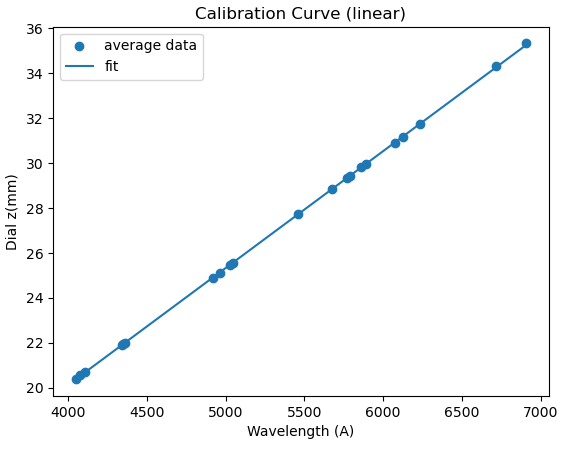
\includegraphics[width=0.9\textwidth]{ccL.png}
    \caption{Calibration plot of the linear regression for calibration.}
    \label{ccL}
\end{minipage}
\hfill
\begin{minipage}{0.48\textwidth}
    \centering
    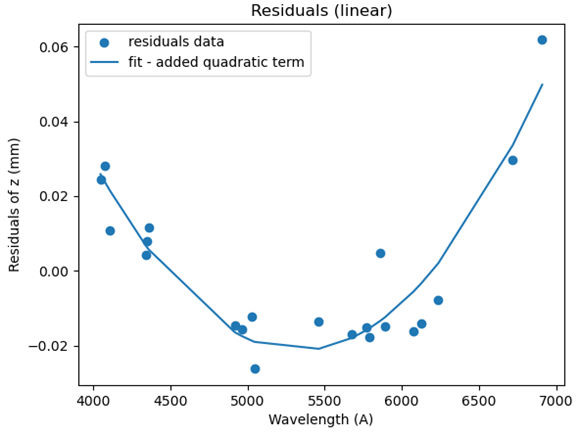
\includegraphics[width=0.9\textwidth]{resL.png}
    \caption{Residual plot of the linear regression for calibration.}
    \label{residual}
\end{minipage}
\end{figure}

It is obvious that the linear model fits the calibration data well, but the residuals show a quadratic pattern. This suggests that we should use a quadratic model to fit the calibration data. We then performed a quadratic regression on the calibration data using Python. The relationship is given by $z = a\lambda^2 + b\lambda + c$, where $a$, $b$ and $c$ are the regression coefficients. The fitted line is shown in figure \ref{ccQ}. The residual plot is shown in figure \ref{residualQ}. The residuals are randomly distributed around zero, indicating that the quadratic model is appropriate for the calibration data.

\begin{figure}[htbp]
\centering
\begin{minipage}{0.48\textwidth}
    \centering
    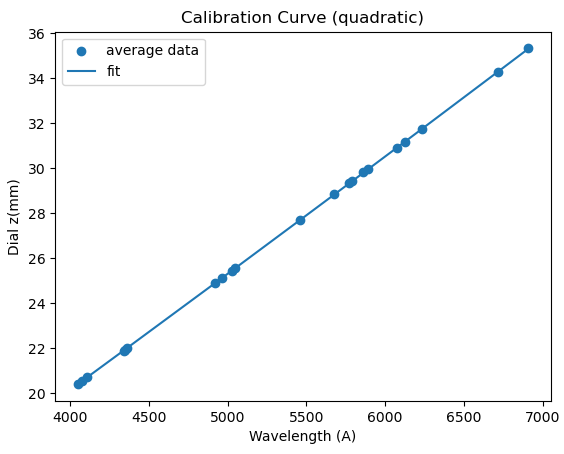
\includegraphics[width=0.9\textwidth]{ccQ.png}
    \caption{Calibration plot of the quadratic regression for calibration.}
    \label{ccQ}
\end{minipage}
\hfill
\begin{minipage}{0.48\textwidth}
    \centering
    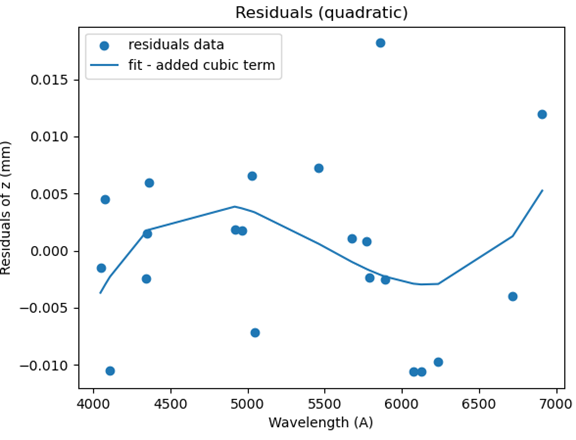
\includegraphics[width=0.9\textwidth]{resQ.png}
    \caption{Residual plot of the quadratic regression for calibration.}
    \label{residualQ}
\end{minipage}
\end{figure}

From figure \ref{residualQ}, we cannot see any pattern in the residuals, which suggests that the quadratic model fits the calibration data correctly. The residuals are distributed around zero, and mostlywithin the range from  -0.01 to 0.01, which is also the smallest resolution of the monochromator. Therefore, we can conclude that the quadratic model is appropriate for the calibration data. $R^2 = 0.999$ also indicates the goodness of fit of the quadratic model.

From the model we can obtain the three coefficients: $a = 2.856(251) \times 10^{-8}$, $b = 4.900(27) \times 10^{-5}$ and $c = 1.017(704) \times 10^{-1}$. These coefficients can be used to convert the micrometer readings of the hydrogen spectrum to wavelengths.



\subsection{Hydrogen wavelengths}

Using the quadratic model obtained from the calibration, we can convert the micrometer readings of the hydrogen spectrum to wavelengths. The results are shown in table \ref{rydberg}.

\begin{table}[htbp]
\centering
\begin{tabular}{c c c c c c}
\hline\hline
Line & $n$ & $z$ (mm) & $\lambda$ (\AA) 
& $R$ ($10^{-3}$\,\AA$^{-1}$) 
& $\sigma_R$ ($10^{-7}$\,\AA$^{-1}$) \\
\hline\hline
$H_\alpha$ & 3 & 33.49(1) & $6560(2)$ & 1.09756 & 3.35 \\
$H_\beta$  & 4 & 24.56(1) & $4852(2)$ & 1.09920 & 4.53 \\
$H_\gamma$ & 5 & 21.90(1) & $4338(2)$ & 1.09772 & 5.06 \\
$H_\delta$ & 6 & 20.64(1) & $4093(2)$ & 1.09944 & 5.37 \\
\hline\hline
\end{tabular}
\caption{Determination of the Rydberg constant from hydrogen spectra}
\label{rydberg}
\end{table}

Since we obtained $\sigma_R$ for each spectral line, a weighted mean of $R$ was calculated. 
The resulting value is

\[
\boxed{R = 1.09828 (22) \times 10^{7}\ \mathrm{m}^{-1}}.
\]

The uncertainty has been rounded to two significant figures, and the central value has been expressed to the corresponding precision.


\subsection{Theoretical prediction}

Given that 
$\varepsilon_0 = 8.8542 \times 10^{-12}\ \mathrm{F\,m^{-1}}$,
$e = 1.6022 \times 10^{-19}\ \mathrm{C}$,
$c = 2.9979 \times 10^{8}\ \mathrm{m\,s^{-1}}$,
$\hbar = 1.0546 \times 10^{-34}\ \mathrm{J\,s} $,
$m_e = 9.1095 \times 10^{-31}\ \mathrm{kg}$,
and $m_p = 1.6726 \times 10^{-27}\ \mathrm{kg}
$, we can calculate the theoretical value of the Rydberg constant using the formula
\[
R_\infty
=
\left( \frac{1}{4\pi\varepsilon_0} \right)^2
\frac{m_e e^4}{4\pi c \hbar^3}
=\boxed{10974000 \ \mathrm{m}^{-1}}.
\]
The Rydberg constant for hydrogen is given by
\[
R_{\mathrm{H}}
=
\left( \frac{1}{4\pi\varepsilon_0} \right)^2
\frac{e^4}{4\pi c \hbar^3}
\frac{m_e m_p}{m_e + m_p}
=\boxed{10968000 \ \mathrm{m}^{-1}}.
\]


\subsection{Result comparisons}

From sections 4.2 and 4.3, we can see that the experimental value of the Rydberg constant is in excellent agreement with theoretical predictions. However, the experimental value is slightly higher than the theoretical $R_{\mathrm{H}}$, making it appear closer to $R_\infty$. We suggest that this small discrepancy ($\sim 0.08\%$) is predominantly driven by systematic errors in the experiment.

Take a constant $\Delta z = +0.04 \text{ mm}$ error in the micrometer reading as an example. If all micrometer readings are overestimated by $\Delta z$, reconsidering the calculation of $R$ we could find the new wavelengths of the hydrogen lines, and then the new Rydberg constant. The results are shown in table \ref{rydberg_corrected_04}. This gives a new weighted mean of $R=1.09665 \times 10^7 \text{ m}^{-1}$, which is much closer to the theoretical $R_{\mathrm{H}}$. 


\begin{table}[htbp]
\centering
\begin{tabular}{c c c c c c}
\hline\hline
Line & $n$ & $z + \Delta z$ (mm) & $\lambda'$ (\AA) 
& $R$ ($10^{-3}$\,\AA$^{-1}$) 
& $\sigma_R$ ($10^{-7}$\,\AA$^{-1}$) \\
\hline\hline
$H_\alpha$ & 3 & 33.53(1) & $6568(2)$ & 1.09622 & 3.34 \\
$H_\beta$  & 4 & 24.60(1) & $4860(2)$ & 1.09739 & 4.52 \\
$H_\gamma$ & 5 & 21.94(1) & $4346(2)$ & 1.09570 & 5.04 \\
$H_\delta$ & 6 & 20.68(1) & $4101(2)$ & 1.09729 & 5.35 \\
\hline\hline
\end{tabular}
\caption{Recalculated Rydberg constant assuming a systematic shift of $\Delta z = +0.04$ mm. }
\label{rydberg_corrected_04}
\end{table}



\section{Conclusion}





\begin{thebibliography}{9}
\bibitem{op13} OP13: The grating monochromator
\end{thebibliography}


\newpage
\section{Appendix}
\begin{table}[htbp]
\centering
\begin{tabular}{c|c|c|c|c}
\hline
\hline
Wavelength (\AA) & Reading 1 (mm) & Reading 2 (mm) & Reading 3 (mm) & Average (mm) \\
\hline\hline
4047.7 & 20.39(1) & 20.39(1) & 20.42(1) & 20.40(1) \\
4079.0 & 20.55(1) & 20.57(1) & 20.58(1) & 20.57(1) \\
4109.2 & 20.69(1) & 20.72(1) & 20.71(1) & 20.71(1) \\
4340.4 & 21.90(1) & 21.92(1) & 21.89(1) & 21.90(1) \\
4348.7 & 21.95(1) & 21.95(1) & 21.95(1) & 21.95(1) \\
4359.5 & 22.00(1) & 22.02(1) & 22.01(1) & 22.01(1) \\
4917.3 & 24.88(1) & 24.89(1) & 24.89(1) & 24.89(1) \\
4961.7 & 25.12(1) & 25.12(1) & 25.11(1) & 25.12(1) \\
5027.0 & 25.46(1) & 25.46(1) & 25.46(1) & 25.46(1) \\
5047.0 & 25.56(1) & 25.54(1) & 25.55(1) & 25.55(1) \\
5462.2 & 27.73(1) & 27.72(1) & 27.72(1) & 27.73(1) \\
5677.4 & 28.84(1) & 28.84(1) & 28.84(1) & 28.84(1) \\
5771.2 & 29.32(1) & 29.33(1) & 29.34(1) & 29.33(1) \\
5792.2 & 29.43(1) & 29.44(1) & 29.44(1) & 29.44(1) \\
5860.9 & 29.82(1) & 29.81(1) & 29.82(1) & 29.82(1) \\
5891.6 & 29.96(1) & 29.95(1) & 29.96(1) & 29.96(1) \\
6074.4 & 30.91(1) & 30.89(1) & 30.92(1) & 30.91(1) \\
6125.2 & 31.17(1) & 31.18(1) & 31.17(1) & 31.17(1) \\
6236.1 & 31.75(1) & 31.75(1) & 31.77(1) & 31.76(1) \\
6718.3 & 34.29(1) & 34.32(1) & 34.30(1) & 34.30(1) \\
6909.4 & 35.33(1) & 35.33(1) & 35.33(1) & 35.33(1) \\
\hline\hline
\end{tabular}
\caption{Spectrometer calibration measurements (mercury lamp)}
\label{calibration}
\end{table}


\begin{table}[H]
\centering
\begin{tabular}{c|c|c|c|c}
\hline
\hline
Spectral Line & Reading 1 (mm) & Reading 2 (mm) & Reading 3 (mm) & Average (mm) \\
\hline\hline
$H_\alpha$ & 33.50(1) & 33.50(1) & 33.48(1) & 33.49(1) \\
$H_\beta$  & 24.57(1) & 24.55(1) & 24.56(1) & 24.56(1) \\
$H_\gamma$ & 21.90(1) & 21.90(1) & 21.91(1) & 21.90(1) \\
$H_\delta$ & 20.66(1) & 20.62(1) & 20.64(1) & 20.64(1) \\
\hline\hline
\end{tabular}
\caption{Spectrometer hydrogen line measurements}
\label{hydrogen}
\end{table}


\begin{figure}[htbp]
\centering
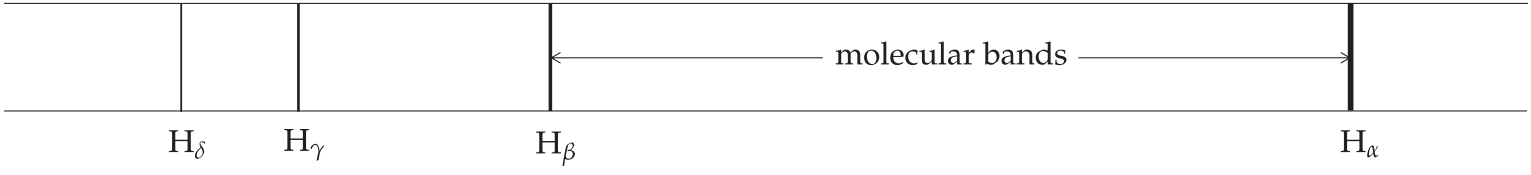
\includegraphics[width=\textwidth]{h.png}
\caption{Corresponding hydrogen spectrum \cite{op13}}
\label{H}
\end{figure}


\end{document}